\begin{figure*}[tb]
  \centering
  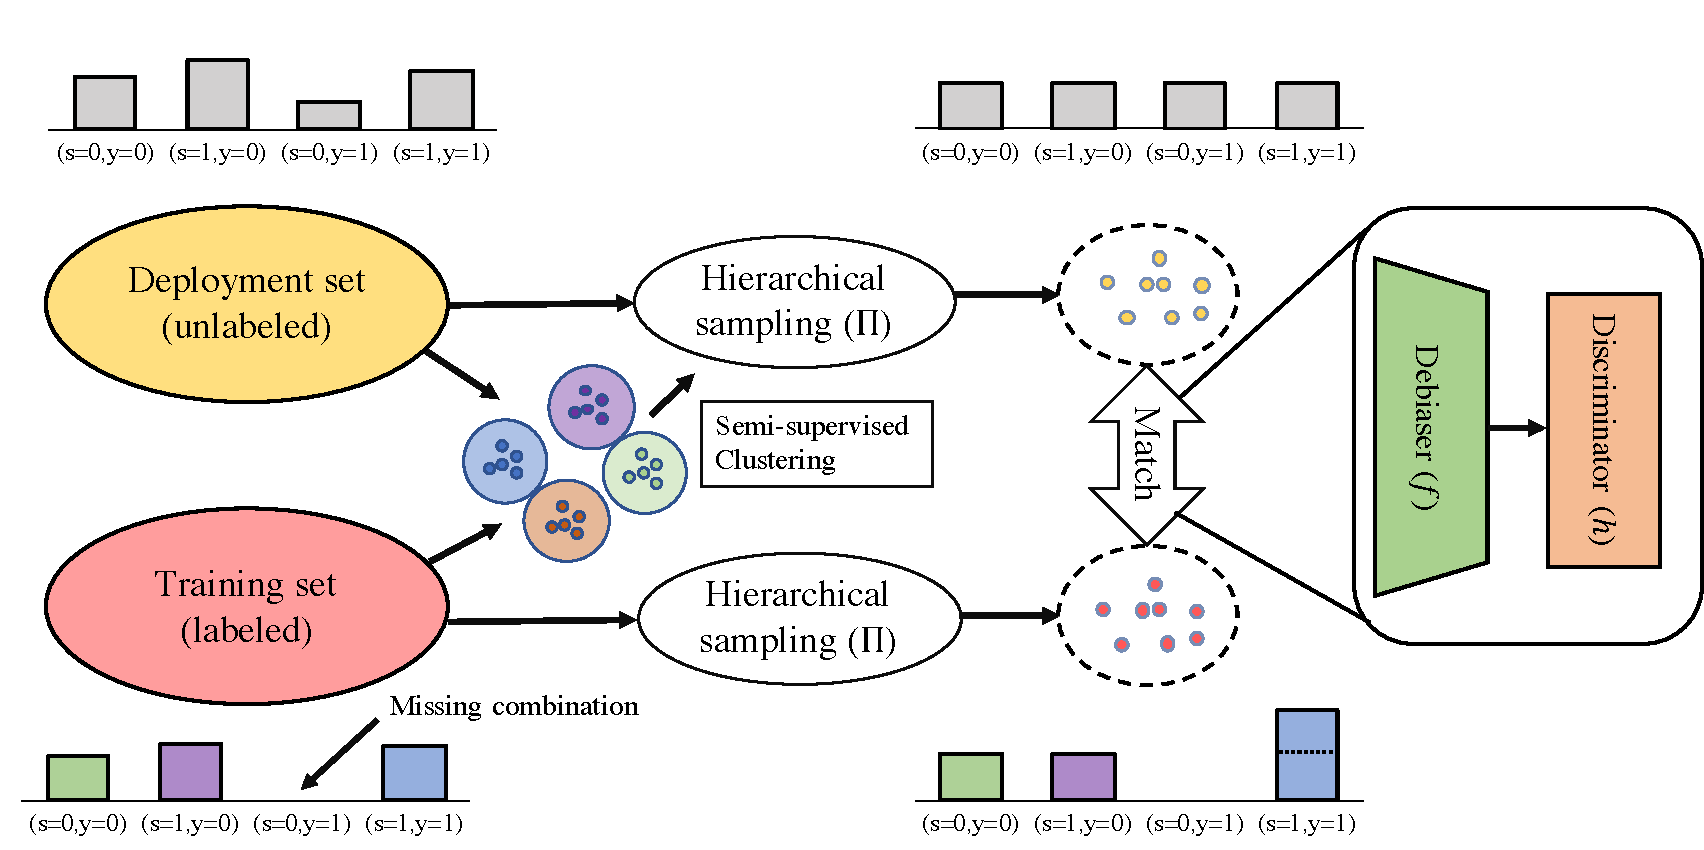
\includegraphics[width=1.0\textwidth]{supmatch/figures/illustrations/pipeline.pdf}
  \caption{%
    Visualisation of our support-matching pipeline.
    % A source is defined as certain combinations of the subgroup, s, and target class, y. Bags are
    % sampled from one of two datasets. The training set has labeled information about both $s$ and
    % $y$ but may be missing support over $S\times Y$. The deployment set on the other hand, is
    % assumed to have full support over $S \times Y$ but is unlabeled, meaning it cannot be used
    % for directly training a classifier. 
    Bags are sampled from the training and deployment sets using the hierarchical sampling
    procedure described in \S\ref{sec:sm-adversarialsm} and defined functionally in
    Eq.~\ref{eq:functional-sampling}. 
    %
    Since we cannot use ground-truth labels for hierarchical sampling of the deployment set, we use
    a semi-supervised clustering algorithm to produce balanced batches. In the event that certain
    combinations are missing, as shown here for $(s=0,y=1)$, the sampling on the training set
    substitutes the missing combinations with combinations that ensure equal representation of the
    target classes. 
    %
    The debiaser is adversarially trained to produce representations from which the source dataset
    cannot be reliably inferred by the discriminator. 
    %
    Assuming the bags are sufficiently balanced and $\gG^\mathit{tr}  \subsetneq \gG=\gS\times\gY$,
    the optimal debiaser is one that produces a representation $z$ that is invariant to $s$, which
    we prove in Appendix~\ref{implication-of-the-objective}.
    }%
  \label{fig:sm-pipeline}
\end{figure*}

